\documentclass[envcountsect, 10pt, portrait, palatino]{beamer}
\usepackage{verbatim}
\usepackage{amsmath}
\usepackage{color}
\usepackage{listings}
%%%%%%%%%%%%%%%%%%%%%%%%%%%%%%% Beamer packages %%%%%%%%%%%%%%%%%%%%%%%
\usetheme{CambridgeUS}
\usefonttheme[onlylarge]{structurebold}
\setbeamerfont*{frametitle}{size=\normalsize,series=\bfseries}
\setbeamertemplate{navigation symbols}{}

\mode<presentation>{
% XXX without this the number does not appear
%\AtBeginDocument{\def\figurename{{\scshape Figure~\thesection.\thefigure}}}
}
% to number captions
\setbeamertemplate{theorems}[ams style]
\setbeamertemplate{caption}[numbered]
%\setbeamertemplate{theorems}[numbered]
%%%%%%%%%%%%%%%%%%%%%%%%%%%% title slide %%%%%%%%%%%%%%%%%%%%%%%%%%%%%%
\title[]{Applied survival analysis}
\author[Constantin T Yiannoutsos]
{ Constantin T Yiannoutsos, Ph.D.}

\date[]{\today}
\newtheorem{defn}{Definition}[section]
\newtheorem{assu}[defn]{Assumption}
\newcommand{\simdot}{\stackrel{\cdot}{\sim}}
\newcommand{\bfbeta}{{\mbox{\boldmath$\beta$}}}
\newcommand{\bfep}{{\mbox{\boldmath$\epsilon$}}}
\newcommand{\bhat}{\hat{\beta}}
\newcommand{\btilde}{\tilde{\mbox{\boldmath$\beta$}}}
\newcommand{\bfmu}{{\mbox{\boldmath$\mu$}}}
\newcommand{\Var}{{\rm Var}}
\newcommand{\Cov}{{\rm Cov}}
\newcommand{\trt}{{\rm trt}}
\newcommand{\pr}{{\rm pr}}
\newcommand{\age}{{\rm age}}
\newcommand{\Sin}{\sum_{i=1}^N}
\newcommand{\Sjn}{\sum_{j=1}^N}
\newcommand{\ui}{{\bf u}_i}
\newcommand{\uj}{{\bf u}_j}
\newcommand{\bfx}{{\mbox{{\bf x}}}}
\newcommand{\bfp}{{\mbox{{\bf p}}}}
\newcommand{\hbfp}{\widehat{\mbox{{\bf p}}}}
\newcommand{\bfy}{{\mbox{{\bf y}}}}
\newcommand{\bfY}{{\mbox{{\bf Y}}}}
\newcommand{\bfZ}{{\mbox{{\bf Z}}}}
\newcommand{\bfa}{{\mbox{{\bf a}}}}
\newcommand{\bfb}{{\mbox{{\bf b}}}}
\newcommand{\bfg}{{\mbox{{\bf g}}}}
\newcommand{\bfU}{{\bf U}}
\newcommand{\bfu}{{\mbox{{\bf u}}}}
\newcommand{\bfz}{{\mbox{{\bf z}}}}
\newcommand{\logit}{{\mbox{{logit}}}}
\newcommand{\bfzero}{{\mbox{{\bf 0}}}}
\newcommand{\hbeta}{{\widehat \beta}}
\newcommand{\heta}{{\widehat \eta}}
\newcommand{\hsigma}{{\widehat \sigma}}
\newcommand{\hmu}{{\widehat \mu}}
\newcommand{\hpi}{{\widehat \pi}}
\newcommand{\cI}{{\cal I}}
\newcommand{\bsigma}{{\bar \sigma}}
\newcommand{\brho}{{\bar \rho}}
\newcommand{\bx}{ {\bar {x} } }
\newcommand{\bY}{ {\bar {Y} } }
\newcommand{\hY}{ {\widehat {Y} } }
\newcommand{\hp}{ {\widehat {p} } }
\newcommand{\hVar}{ {\widehat {Var} } }

\setlength{\baselineskip}{2.5em}
% The main document
\begin{document}
\begin{frame}
  \titlepage
\end{frame}
%%%%%%%%%%%%%%%%%%%%%%%%%%%%%%%%%%%%%%%%%%%%%%%%%%%%%%%%%%%%%%%%%%%%%%%
\begin{frame}{Contents of today's lecture}
  \tableofcontents
\end{frame}
\section{Assessing the PH assumption}
\subsection{Introduction}
\begin{frame}{Assessing the PH Assumption}
So far, we've been considering the following Cox PH model:
\begin{eqnarray*}
\lambda(t,\mathbf{Z}) = \lambda_0(t) ~ \exp(\mathbf{\beta} \mathbf{Z})
                  = \lambda_0(t) ~\exp\left(\sum \beta_j Z_j\right)
\end{eqnarray*}
where $\beta_j$ is the parameter for the the $j$-th covariate ($Z_j$).
\end{frame}
\begin{frame}{ Important features of this model:}
\begin{itemize}
\item[(1)] the baseline hazard depends on $t$, but not on the covariates
$Z_1,...,Z_p$
\item[(2)] the hazard ratio, i.e., $\exp(\mathbf{\beta} \mathbf{Z})$, depends on
the covariates $\mathbf{Z}=(Z_1,...,Z_p)$, but not on time $t$.
\end{itemize}

Assumption (2) is what led us to call this a proportional
hazards model.  That's because we could take the ratio of the
hazards for two individuals with covariates $\mathbf{Z}_{i}$ and
$\mathbf{Z}_{i'}$, and write it as a constant in terms of the covariates.
\end{frame}
\subsection{The proportional Hazards Assumption}
\begin{frame}{ Hazard Ratio:}
\begin{eqnarray*}
\frac{\lambda(t,{\mathbf{Z}_i})}{\lambda(t,{\mathbf{Z}_{i'}})} & = &
\frac{\lambda_0(t) \exp(\mathbf{\beta} \mathbf{Z}_i)}
{\lambda_0(t) \exp(\mathbf{\beta} \mathbf{Z}_{i'})}\\[2ex]
& = & \frac{\exp(\mathbf{\beta} \mathbf{Z}_i)}
{\exp(\mathbf{\beta} \mathbf{Z}_{i'})}\\[2ex]
& = & \exp[\mathbf{\beta} (\mathbf{Z}_i - \mathbf{Z}_{i'})]\\[2ex]
& = & \exp[\sum \beta_j (Z_{ij} - Z_{i'j})] ~=~ \theta
\end{eqnarray*}
\end{frame}
\begin{frame}
In the last formula, $Z_{ij}$ is the value of the $j$-th covariate
for the $i$-th individual.  For example, $Z_{42}$ might be the value
of {\sc gender} (0 or 1) for the the 4-th person.

\vspace{0.3in}
We can also write the hazard for the $i$-th person as a constant
times the hazard for the $i'$-th person:
\begin{eqnarray*}
\lambda(t,{\mathbf{Z}_i}) & = & \theta ~ \lambda(t,{\mathbf{Z}_{i'}})
\end{eqnarray*}
Thus, the HR between two types of individuals is constant (i.e., =$\theta$)
over time.  These are mathematical ways of stating the proportional
hazards assumption.
%%%%%%%%%%%%%%%%%%%%%%%%%%%%%%%%%%%%%%%%%%%%%%%%%%%%%%%%%%%%%%%%%%%%%%%%%%%%
\end{frame}
\begin{frame}{Ways to check the PH assumption}
There are several options for checking the assumption of
proportional hazards:

\begin{itemize}
\item[I.] {\bf Graphical}
\begin{itemize}
\item[(a)] Plots of survival estimates for two subgroups
\item[(b)] Plots of $\log[-\log(\hat{S})]$ vs $\log(t)$ for two subgroups
\item[(c)] Plots of weighted Schoenfeld residuals vs time
\item[(d)] Plots of observed survival probabilities versus expected under
PH model (see Kleinbaum, ch.4)
\end{itemize}

\item[II.] {\bf Use of goodness of fit tests} - we can construct a
goodness-of-fit test based on comparing the observed survival
probability (from {\tt sts list}) with the expected (from {\tt stcox})
under the assumption of proportional hazards - see Kleinbaum ch.4

\item[III.] {\bf Including interaction terms between a covariate and $t$}
(time-dependent covariates)
\end{itemize}
\end{frame}
\begin{frame}{ How do we interpret the above?}

Kleinbaum (and other texts) suggest a strategy of assuming that PH
holds unless there is very strong evidence to counter this assumption:
\begin{itemize}
\item estimated survival curves are fairly separated, then cross
\item estimated log cumulative hazard curves cross, or look very
unparallel over time
\item weighted Schoenfeld residuals clearly increase or decrease over
time (you could fit a OLS regression line and see if the slope is
significant)
\item test for time $\times$ covariate interaction term is significant
(this relates to time-dependent covariates)
\end{itemize}
\end{frame}
\begin{frame}{What if the PH model does not hold?}
If PH doesn't exactly hold for a particular covariate but we fit the
PH model anyway, then what we are getting is sort of an average HR,
averaged over the event times.
\\[2ex]
In most cases, this is not such a bad estimate.  Allison claims that
too much emphasis is put on testing the PH assumption, and not enough
to other important aspects of the model.
%%%%%%%%%%%%%%%%%%%%%%%%%%%%%%%%%%%%%%%%%%%%%%%%%%%%%%%%%%%%%%%%%%%%%%%%%%%%
\end{frame}
\begin{frame}{ Implications of proportional hazards}

Consider a PH model with a single covariate, Z:

\[   \lambda(t; Z)  = \lambda_0(t) e^{\beta Z} \]


What does this imply for the relation between the survivorship
functions at various values of Z?
\\[2ex]
Under PH,
\[  \log[-\log[S(t;Z)]] =  \log[-\log[S_0(t)]] + \beta Z \]
\end{frame}
\begin{frame}{Implications for the cumulative hazard}
In general, we have the following relationship:
\begin{eqnarray*}
\Lambda_i(t) & = & \int_0^t \lambda_i(u) du\\[1ex]
             & = & \int_0^t \lambda_0(u) \exp(\mathbf{\beta}\mathbf{Z}_i) du\\[1ex]
             & = & \exp(\mathbf{\beta}\mathbf{Z}_i) \, \int_0^t \lambda_0(u) du\\[1ex]
             & = & \exp(\mathbf{\beta}\mathbf{Z}_i) \, \Lambda_0(t)
\end{eqnarray*}

This means that the ratio of the cumulative hazards is the same
as the ratio of hazard rates:
\begin{eqnarray*}
\frac{\Lambda_i(t)}{\Lambda_0(t)} & = & \exp(\mathbf{\beta}\mathbf{Z}_i)
~=~ \exp(\beta_1 Z_{1i} + \cdots + \beta_p Z_{pi})
\end{eqnarray*}
%%%%%%%%%%%%%%%%%%%%%%%%%%%%%%%%%%%%%%%%%%%%%%%%%%%%%%%%%%%%%%%%%%%%%%%%%%%%
\end{frame}
\begin{frame}{Implications for the linear predictor}
Using the above relationship, we can show that:
\begin{eqnarray*}
\mathbf{\beta}\mathbf{Z}_i & = & \log \left(\frac{\Lambda_i(t)}{\Lambda_0(t)}\right)\\[2ex]
& = & \log \Lambda_i(t) - \log \Lambda_0(t)  \\[2ex]
& = & \log[-\log S_i(t)] - \log[-\log S_0(t)]  \\[2ex]
\mbox{so}~~ \log[-\log S_i(t)] & = & \log[-\log S_0(t)] + \mathbf{\beta}\mathbf{Z}_i
\end{eqnarray*}
\end{frame}
\begin{frame}{What is the bottom line?}
Thus, to assess if the hazards are actually proportional to each other
over time
\begin{itemize}
\item  calculate Kaplan Meier Curves for various levels of $Z$
\item  compute $\log[-\log(\hat{S}(t;Z))]$ (i.e., log cumulative hazard)
\item  plot vs log-time to see if they are parallel (lines or curves)
\end{itemize}
Note:  If $Z$ is continuous, break into categories.
%%%%%%%%%%%%%%%%%%%%%%%%%%%%%%%%%%%%%%%%%%%%%%%%%%%%%%%%%%%%%%%%%%%%%%%%%%%%
\end{frame}
\begin{frame}{Some ideas}

{\bf Question:}  Why not just compare the underlying hazard rates to
see if they are proportional?
\\[2ex]
Here's two simulated examples with hazards which are truly
proportional between the two groups:
\begin{center}
\begin{tabular}{cc}
{\bf Weibull-type hazard} & {\bf U-shaped hazard}\\
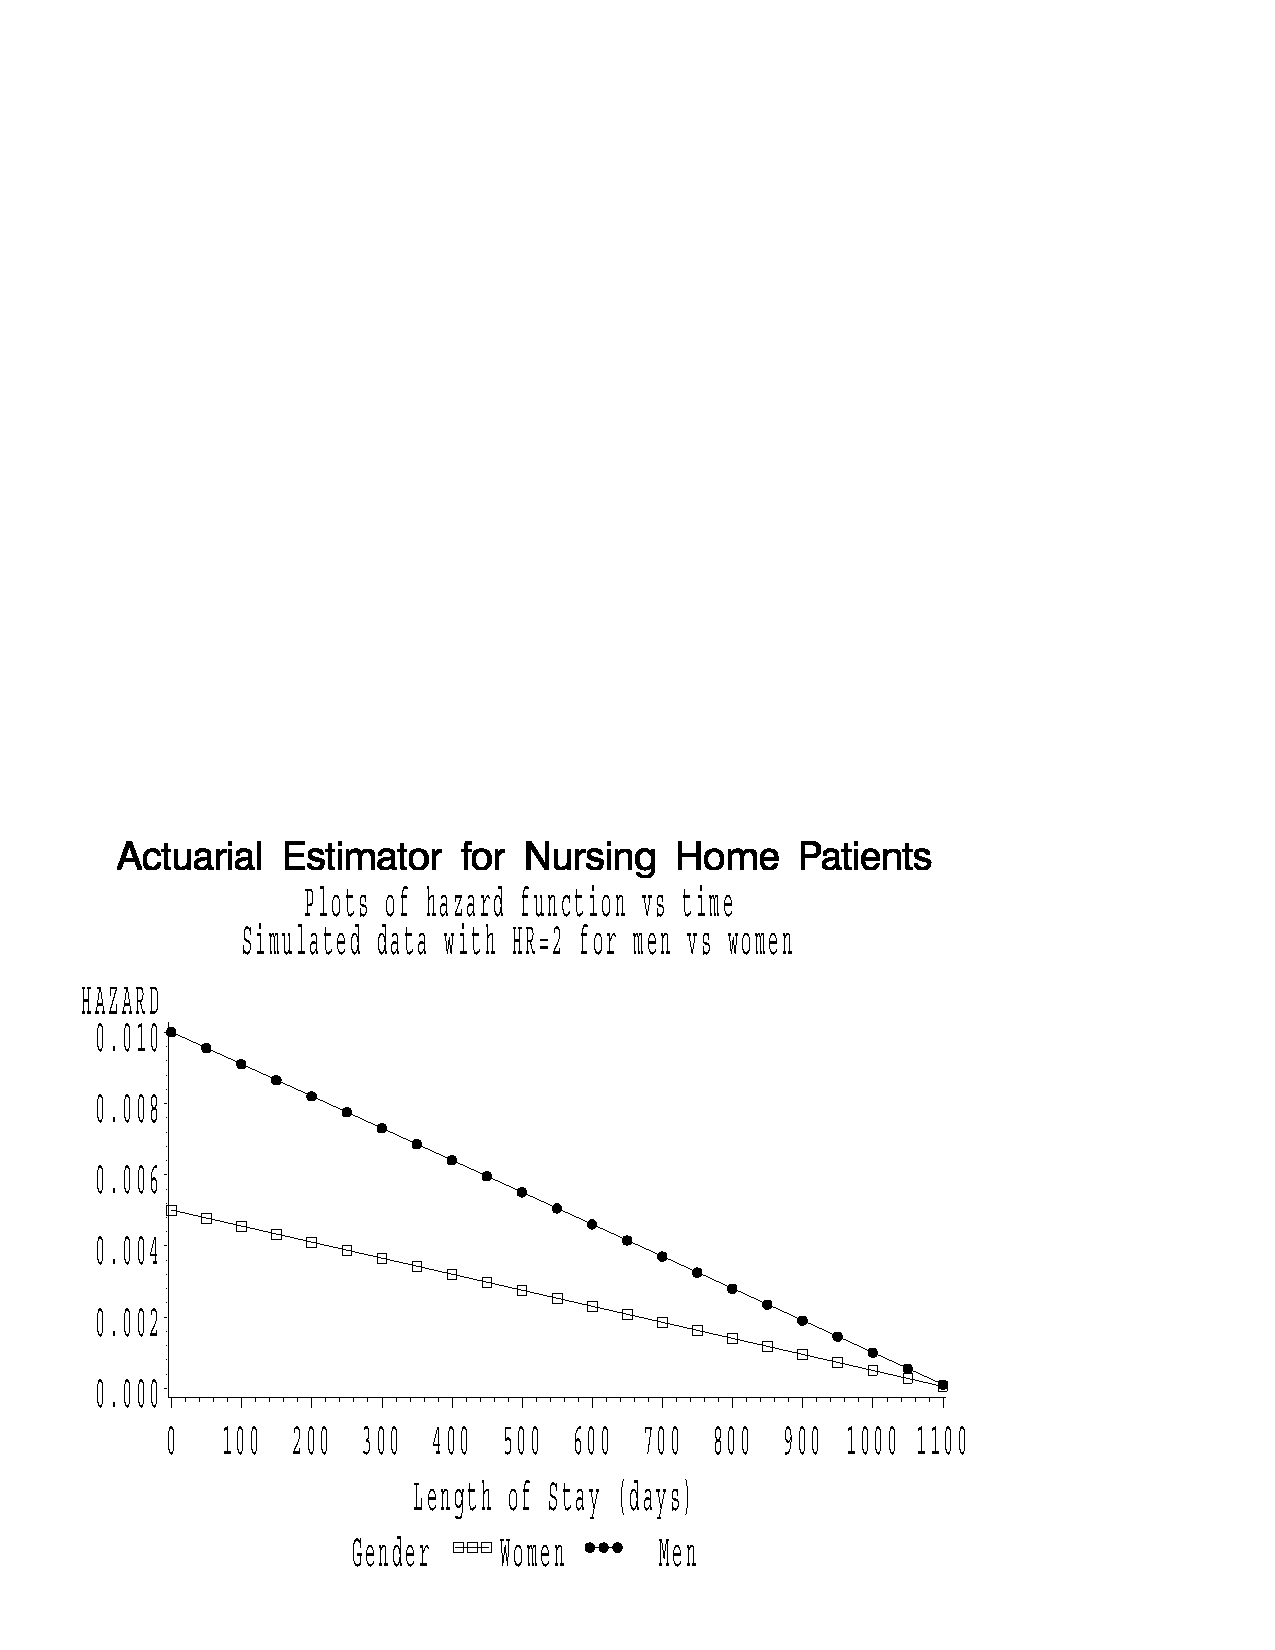
\includegraphics[width=2in]{hazards_sim1.pdf} &
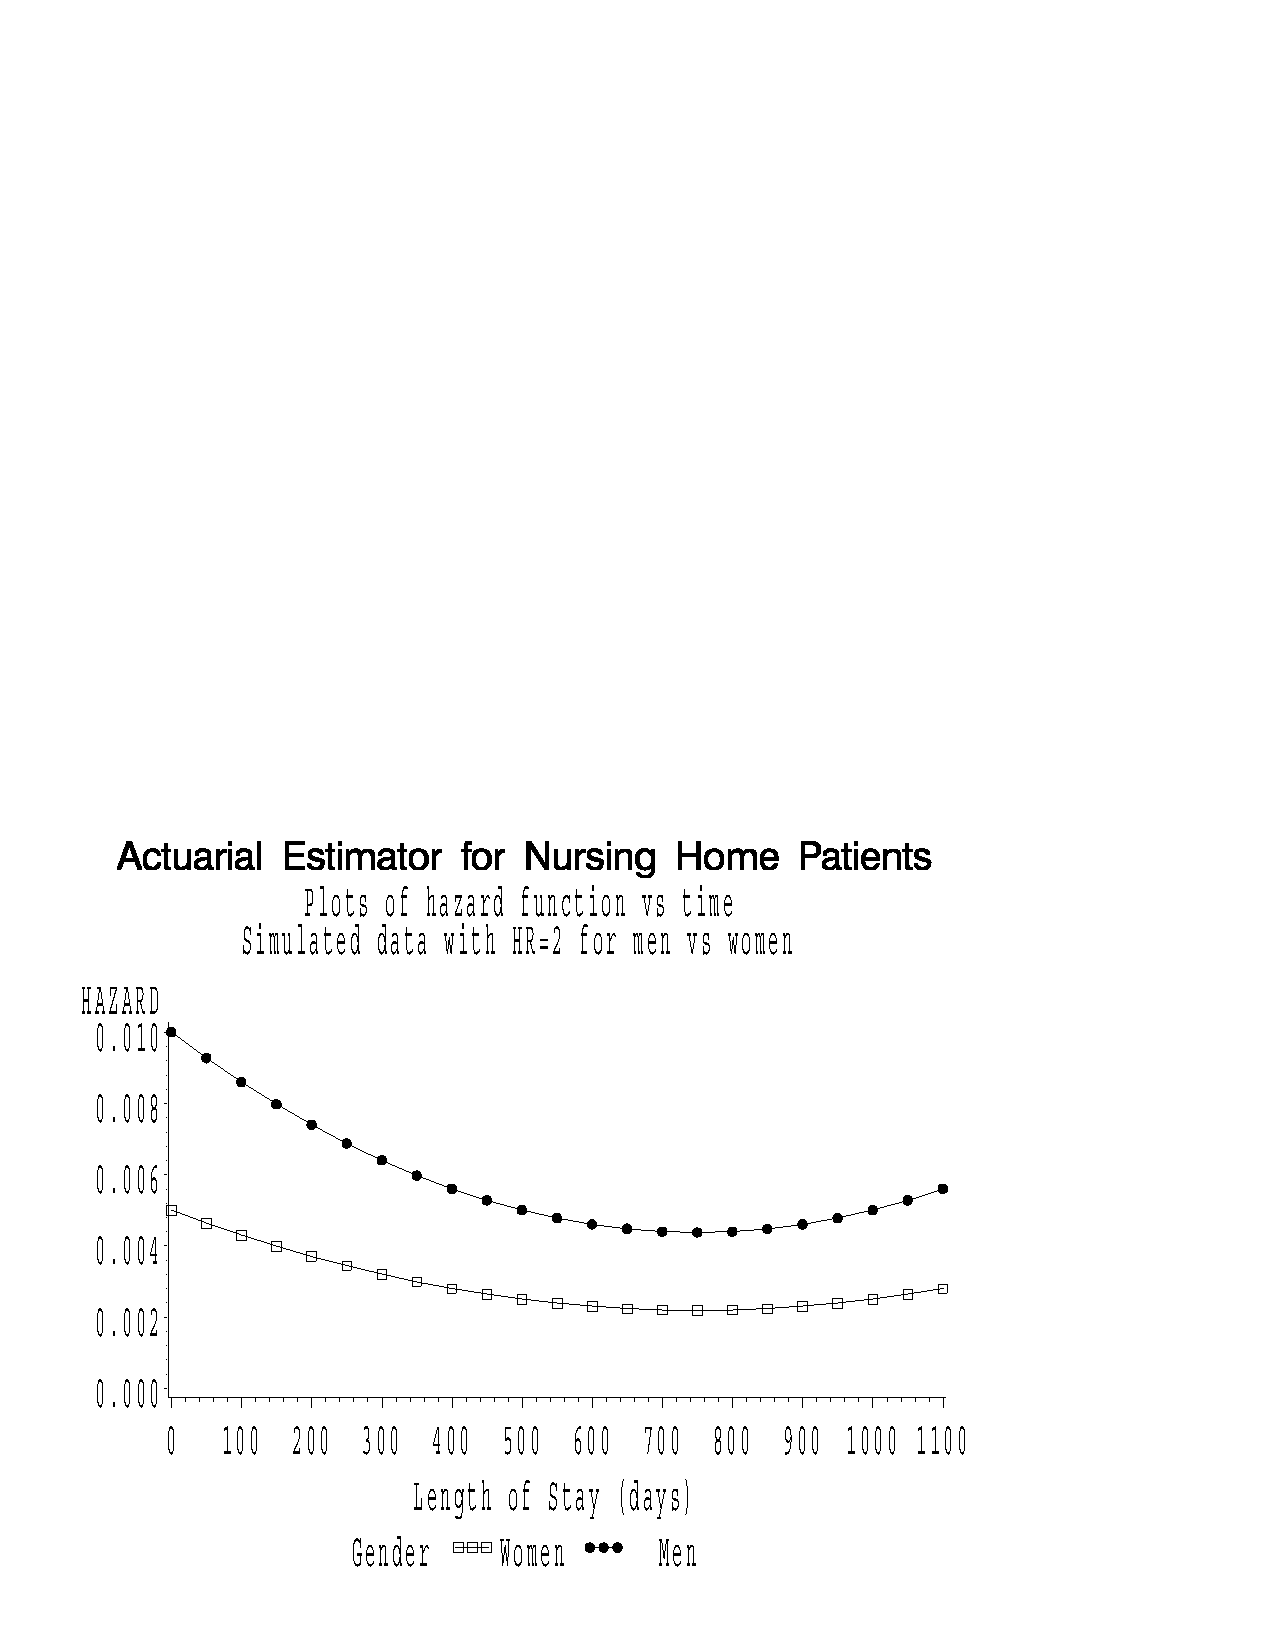
\includegraphics[width=2in]{hazards_sim2.pdf}
\end{tabular}
\end{center}
\end{frame}
\begin{frame}

{\bf Reason 1:} It's hard to eyeball these figures and see that
the hazard rates are proportional - it would be easier to look for
a constant shift between lines.~\\[2ex]

{\bf Reason 2:} Estimated hazard rates tend to be more unstable than the
cumulative hazard rate.
\end{frame}
\begin{frame}{Example: Nursing home data}

Consider the nursing home example (where we think PH is reasonable).
\\[2ex]
If we group the data into intervals and calculate the hazard rate using
actuarial method, we get these plots:

\begin{center}
\begin{tabular}{cc}
{\bf 200 day intervals} & {\bf 100 day intervals}\\
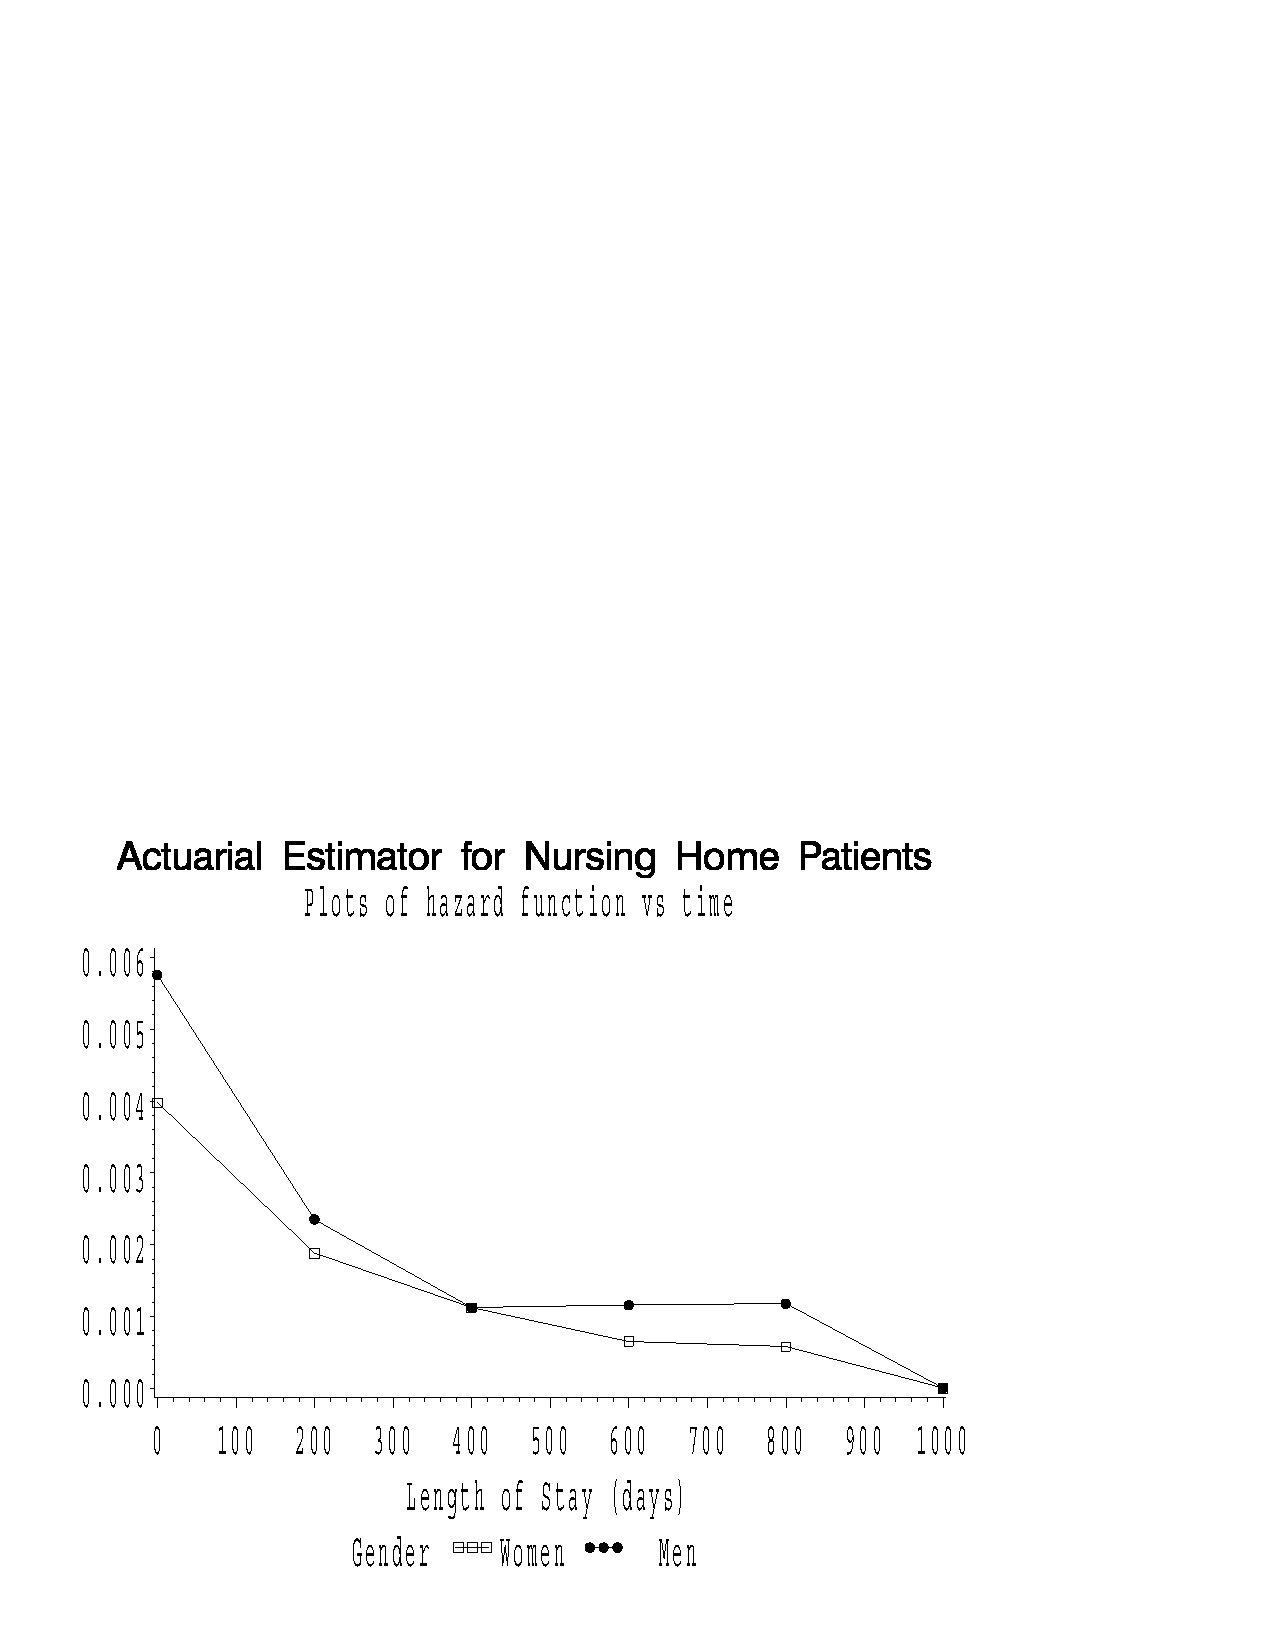
\includegraphics[width=2in]{hazards_nh1.pdf} &
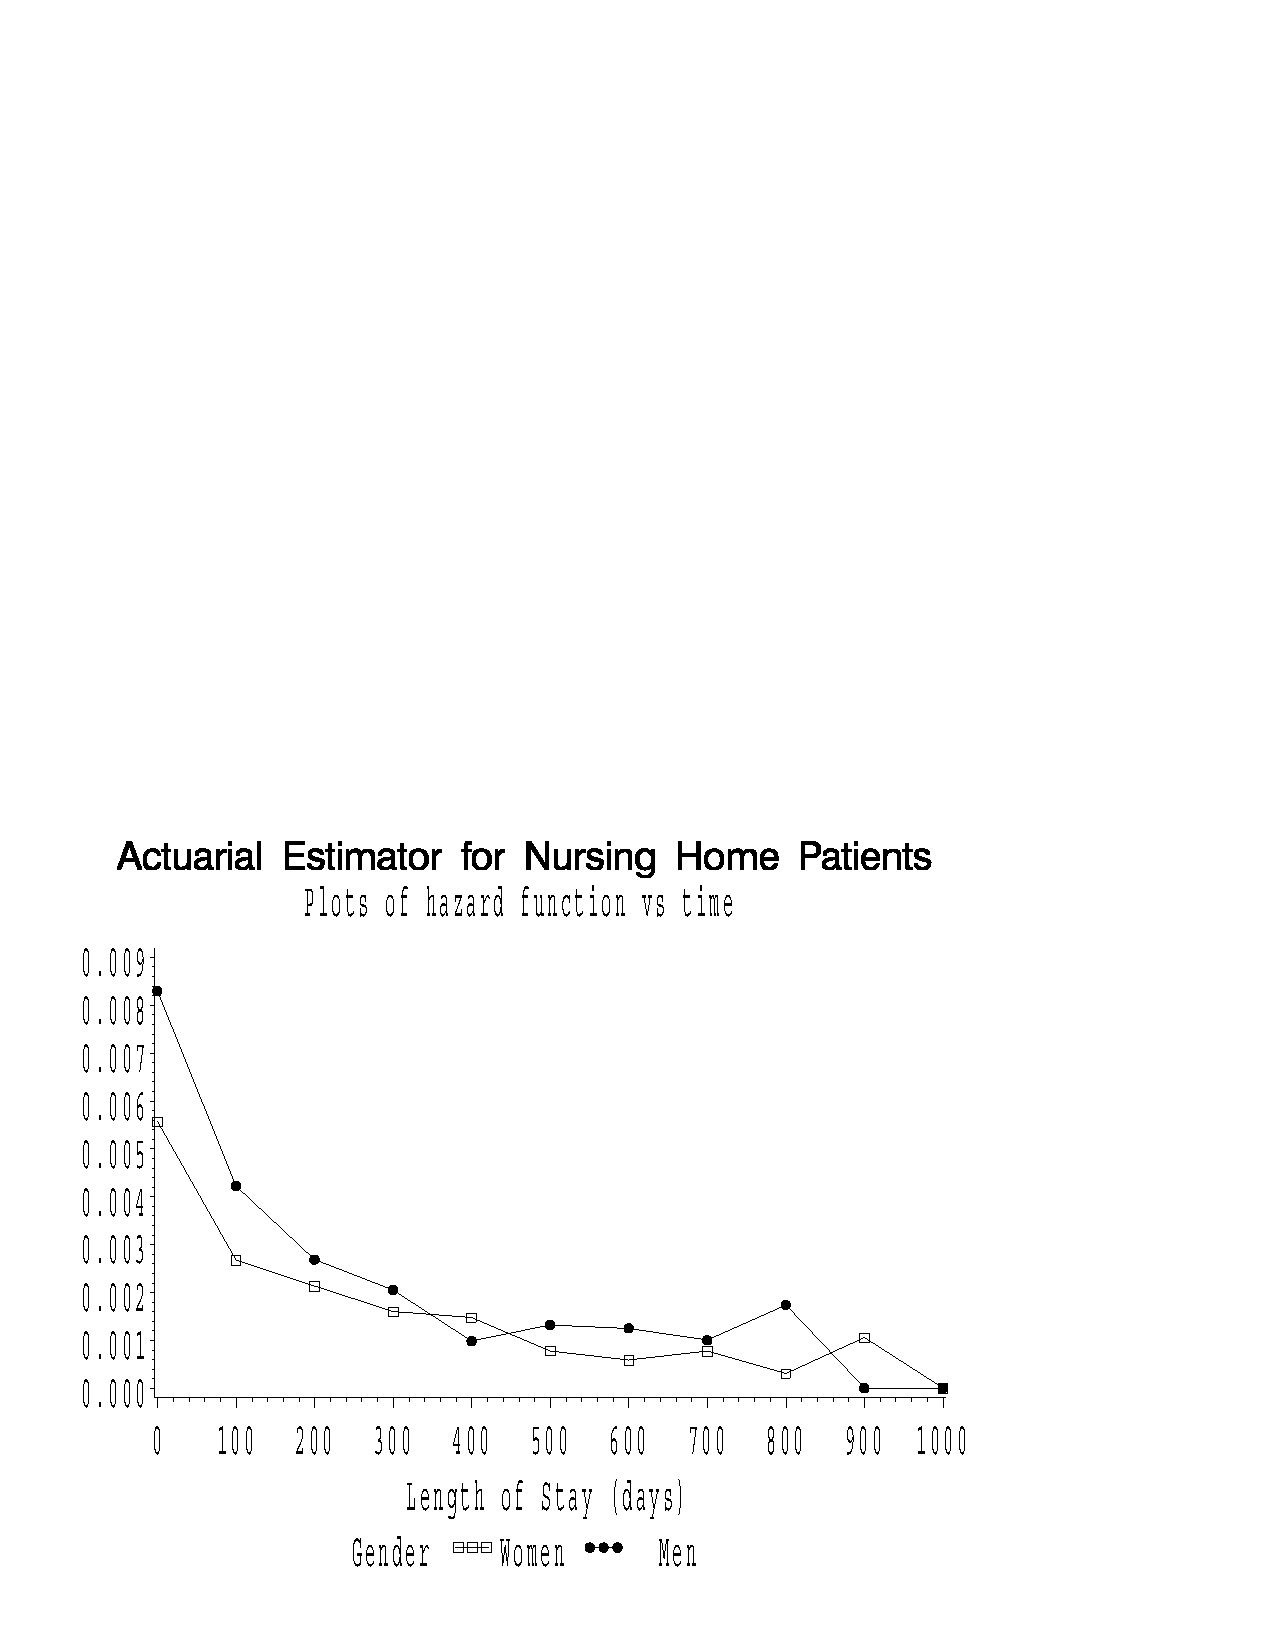
\includegraphics[width=2in]{hazards_nh2.pdf}
\end{tabular}
\end{center}
\end{frame}
\begin{frame}
\begin{center}
\begin{tabular}{cc}
{\bf 50 day intervals} & {\bf 25 day intervals}\\
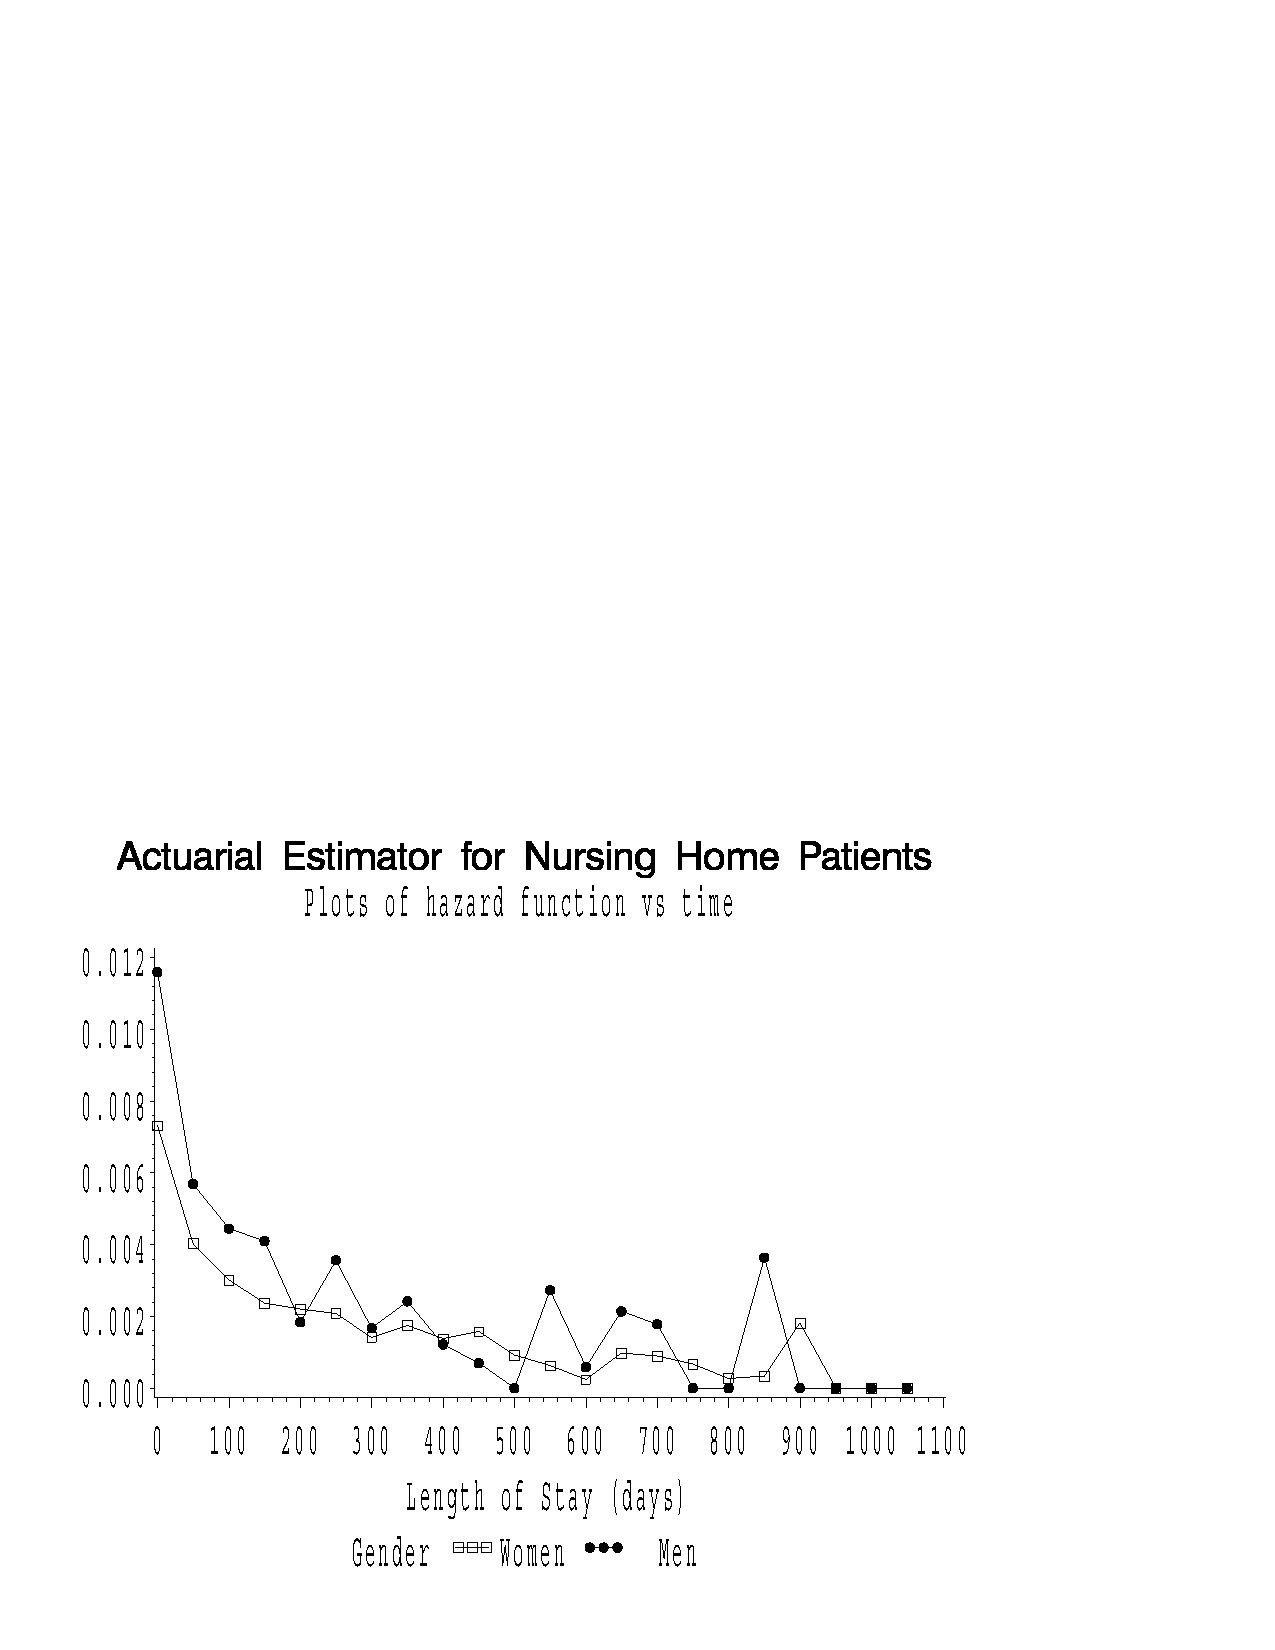
\includegraphics[width=2in]{hazards_nh3.pdf} &
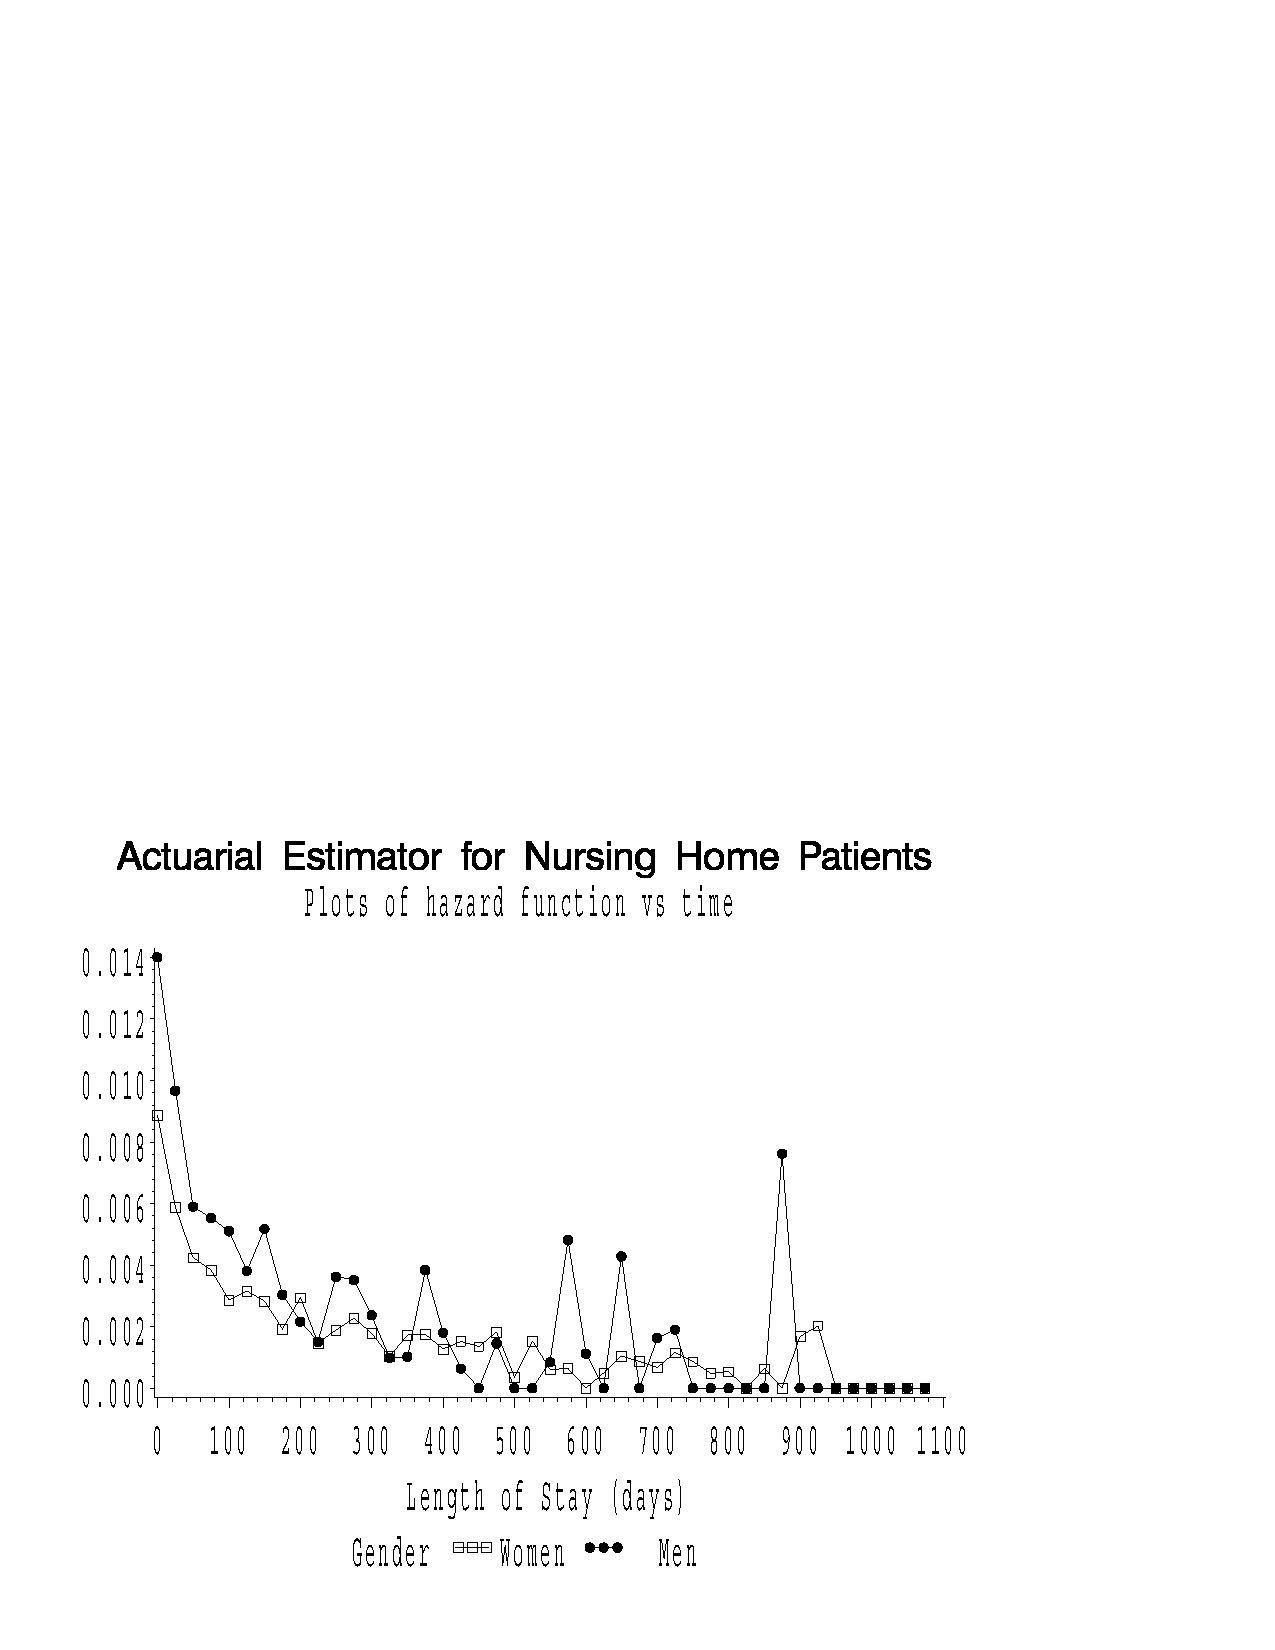
\includegraphics[width=2in]{hazards_nh4.pdf}
\end{tabular}
\end{center}
In contrast, the log cumulative hazard plots are easier to
interpret and tend to give more stable estimates.
\end{frame}
\subsection{Log-log(survival) plots as visual checks of the model fit}
\begin{frame}[fragile]{Example: Nursing Home - gender}

\scriptsize
\begin{verbatim}
fitKMgen = survfit( Surv(los,fail) ~ gender,data = nurshome)

plot(fitKMgen, mark.time = F, fun = "cloglog",
     xlab = "Length of Stay (days on a log-scale)", ylab = "Ln[-Ln(Survival Probabilities)]",
     lty = 1:2,col = c("blue","red"))
legend("topleft",lty = 1:2,col = c("blue","red"),bty="n",legend = c("Female","Male"))
\end{verbatim}
%\end{frame}
%\begin{frame}{Example: Assessment of the PH assumption for {\tt gender}}
%\normalsize
\vspace*{-.25in}
%The results are as follows:
\centerline{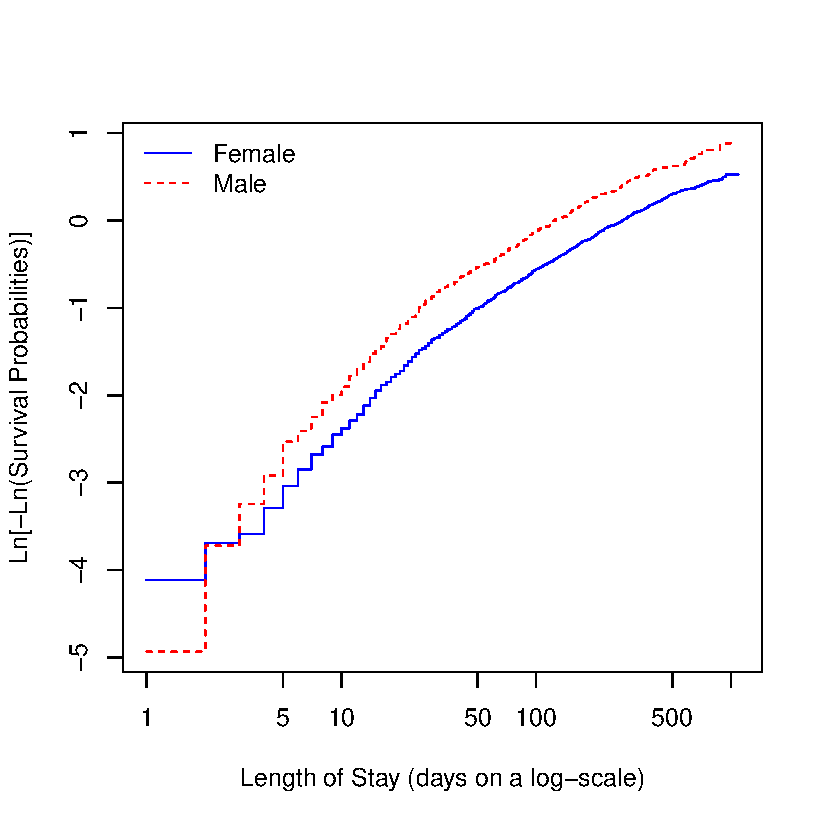
\includegraphics[width=2.5in]{ch12ph_sex.pdf}}
\normalsize
\end{frame}
\begin{frame}{Example: Nursing Home - marital status}
A similar situation is the case with respect to the effect of marital status;
~\\[-1ex]
\vspace*{-.25in}
\centerline{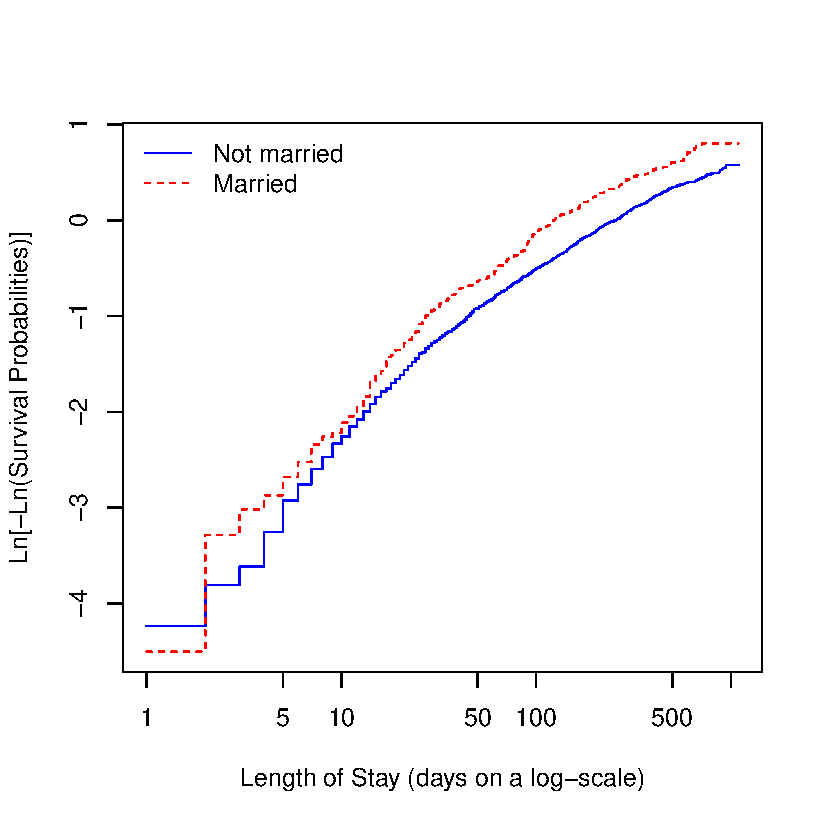
\includegraphics[width=2.5in]{ch12ph_mar_status.pdf}}
This is equivalent to comparing plots of the log cumulative
hazard, $\log(\hat\Lambda(t))$, between the covariate levels, since
\[ \Lambda(t) =  \int_0^t \lambda(u; Z)du = -\log[S(t)]   \]
%%%%%%%%%%%%%%%%%%%%%%%%%%%%%%%%%%%%%%%%%%%%%%%%%%%%%%%%%%%%%%%%%%%%%%%%%%%%
\end{frame}
\subsection{Assessing the PH assumption with multiple covariates}
\begin{frame}{Assessing proportionality with several covariates}

If there are enough data and you only have a couple of
covariates, create a new covariate that takes a different value for
every combination of covariate values.
\\[2ex]
If there are too many covariates (or not enough data) for
this, then there is a way to test proportionality for
each variable, one at a time, using the stratification option.
\end{frame}
\begin{frame}[fragile]{ Example: Health status and gender for nursing home data.}

\scriptsize
\begin{verbatim}
nurshome$hlthsex = c( 1*(nurshome$gender==0 & nurshome$health==2) +
                      2*(nurshome$gender==1 & nurshome$health==2) +
                      3*(nurshome$gender==0 & nurshome$health==5) +
                      4*(nurshome$gender==1 & nurshome$health==5) )
\end{verbatim}
~\\[-2ex]
\vspace*{-.25in}
\centerline{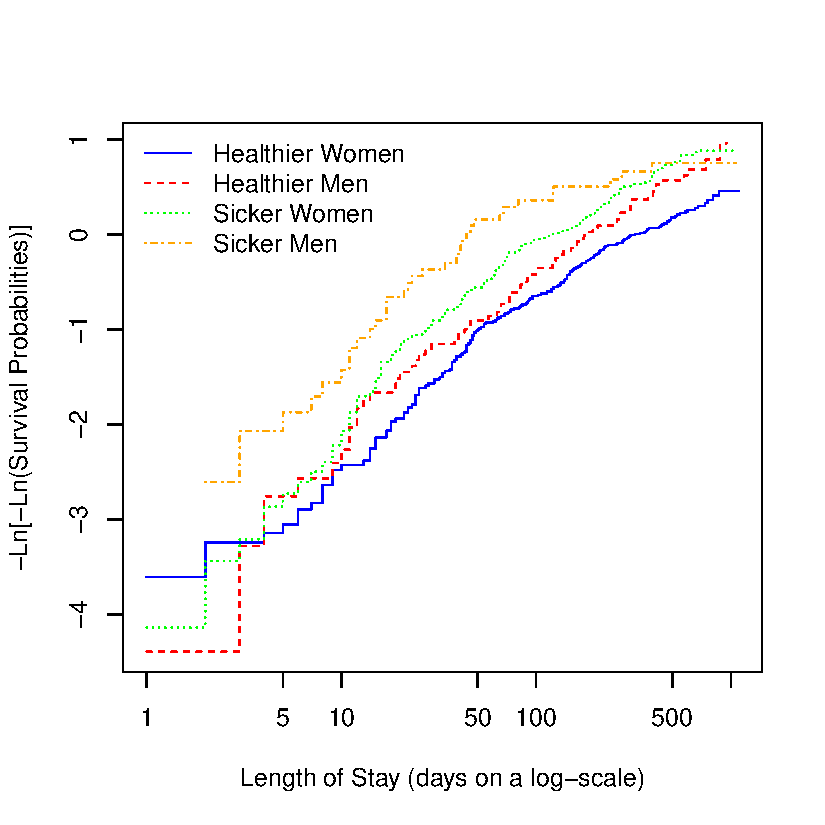
\includegraphics[width=2.5in]{ch12ph_hlthsex.pdf}}
\normalsize
%%%%%%%%%%%%%%%%%%%%%%%%%%%%%%%%%%%%%%%%%%%%%%%%%%%%%%%%%%%%%%%%%%%%%%%%%%%%
\end{frame}
\subsection{When the PH assumption does not hold}
\begin{frame}{What if proportional hazards fails?}
If the PH assumption fails, we can do any of the following:
\begin{itemize}
\item do a stratified analysis

\item include a time-varying covariate to
       allow changing  hazard ratios over time

\item include interactions with time
\end{itemize}

The second these two options relate to time-dependent covariates,
which is something we will cover later in this course.
\\[2ex]
We will focus on the first alternative, and then the second
two options will be briefly described.
%%%%%%%%%%%%%%%%%%%%%%%%%%%%%%%%%%%%%%%%%%%%%%%%%%%%%%%%%%%%%%%%%%%%%%%%%%%%
\end{frame}
\begin{frame}{Stratified Analyses}

Suppose:
\begin{itemize}
\item we are happy with the proportionality assumption on $Z_1$
\item proportionality simply does not hold between various
levels of a second variable  $Z_2$.
\end{itemize}

If $Z_2$ is discrete (with $a$ levels) and there are enough data,
fit the following {\bf stratified model}:

\[   \lambda(t; Z_1, Z_2)  = \lambda_{Z_2}(t) e^{\beta Z_1} \]

For example, a new treatment might lead to a 50\% decrease
in hazard of death versus the standard treatment, but the
hazard for standard treatment might be different for
each hospital.
\\[2ex]
{\bf A stratified model can be useful both for primary analysis
and for checking the PH assumption.}
%%%%%%%%%%%%%%%%%%%%%%%%%%%%%%%%%%%%%%%%%%%%%%%%%%%%%%%%%%%%%%%%%%%%%%%%%%%%
\end{frame}
\begin{frame}{Assessing PH assumption for several covariates}

Suppose we have several covariates $(\mathbf{Z}=  Z_1$,  $Z_2$, ... $Z_p$),
and we want to know if the following PH model holds:

\[ \lambda(t; {\mathbf{Z}})  = \lambda_0(t)~ e^{\beta_1 Z_1 + ... + \beta_p Z_p} \]

To start, we fit a model which stratifies by $Z_k$:

\[ \lambda(t; {\mathbf{Z}})  = \lambda_{0Z_k}(t) ~e^{\beta_1 Z_1 + ... +
\beta_{k-1} Z_{k-1} + \beta_{k+1} Z_{k+1} +...+ \beta_p Z_p} \]

Since we can estimate the survival function for any subgroup, we can
use this to estimate the baseline survival function,
$S_{0Z_k}(t)$, for each level of $Z_k$.
\\[2ex]
Then we compute $- \log S(t)$ for each level of $Z_k$,
controlling for the other covariates in the model, and
graphically check whether the log cumulative hazards are parallel
across strata levels.
%%%%%%%%%%%%%%%%%%%%%%%%%%%%%%%%%%%%%%%%%%%%%%%%%%%%%%%%%%%%%%%%%%%%%%%%%%%%
\end{frame}
\begin{frame}{Example: PH assumption for {\tt gender} (in the nursing home data)}
To assess the PH assumption for gender we do the following:
\begin{itemize}
\item  include {\tt married} and {\tt health} as covariates in
a Cox PH model, but {\em stratify} by {\tt gender}.
\item calculate the baseline survival function for each level of
the variable {\tt gender} (i.e., males and females)
\item  plot the log-cumulative hazards for males and females and
evaluate whether the lines (curves) are parallel
\end{itemize}

In the above example, we make the PH assumption for {\tt married} and
{\tt health}, but not for {\tt gender}.
\\[2ex]
This is like getting a KM survival estimate for each gender without
assuming PH, but is more flexible since we can control for other covariates.
\\[2ex]
We would repeat the stratification for each variable for which we
wanted to check the PH assumption.
%%%%%%%%%%%%%%%%%%%%%%%%%%%%%%%%%%%%%%%%%%%%%%%%%%%%%%%%%%%%%%%%%%%%%%%%%%%%
\end{frame}
\begin{frame}[fragile]{R Code for assesing the PH assumption within a stratified model}

\scriptsize
\begin{verbatim}
fit.strat <- coxph( Surv(los,fail) ~ married + health + strata(gender),data = nurshome)
summary(fit.strat)

Call:
coxph(formula = Surv(los, fail) ~ married + health + strata(gender),
    data = nurshome)

  n= 1591, number of events= 1269

           coef exp(coef) se(coef)     z Pr(>|z|)
married 0.16101   1.17470  0.07720 2.086    0.037 *
health  0.16897   1.18408  0.03128 5.402  6.6e-08 ***
---
Signif. codes:  0 ‘***’ 0.001 ‘**’ 0.01 ‘*’ 0.05 ‘.’ 0.1 ‘ ’ 1

        exp(coef) exp(-coef) lower .95 upper .95
married     1.175     0.8513     1.010     1.367
health      1.184     0.8445     1.114     1.259

Concordance= 0.55  (se = 0.011 )
Rsquare= 0.021   (max possible= 1 )
Likelihood ratio test= 33.97  on 2 df,   p=4.199e-08
Wald test            = 34.22  on 2 df,   p=3.702e-08
Score (logrank) test = 34.33  on 2 df,   p=3.518e-08
\end{verbatim}
\end{frame}
\begin{frame}[fragile]{Log[-log(survival)] plots for gender {\bf Controlling for Marital and Health Status}}

\scriptsize
\begin{verbatim}
fitCoxgen2 = survfit(fit.strat)

plot(fitCoxgen2,mark.time = F,ylab = "-Ln[-Ln(Survival Probabilities)]",fun = "cloglog",
     xlab = "Length of Stay (days on a log-scale)",lty = 1:2,col = c("blue","red"))
legend("topleft",lty = 1:2,col = c("blue","red"),bty = "n",
       legend = c("Female","Male"))
\end{verbatim}
\end{frame}

\begin{frame}{Stratified model controlling for health and marital status}
\centerline{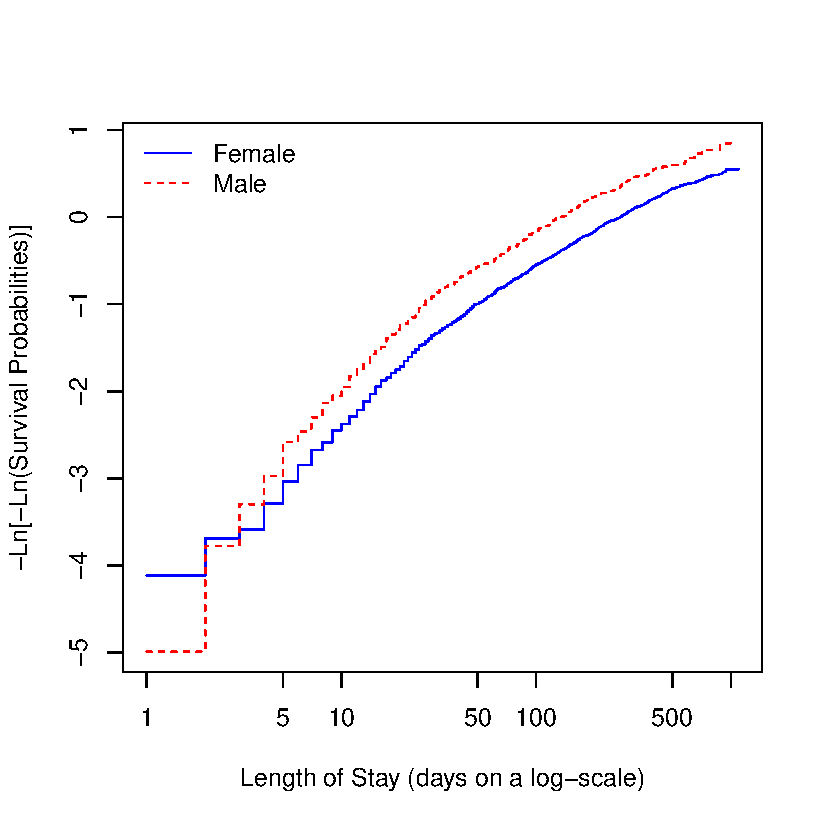
\includegraphics[width=3in]{ch12stratph.pdf}}
\end{frame}
\begin{frame}{Models with time-dependent Interactions}

Consider a PH model with two covariates $Z_1$ and $Z_2$.
The standard PH model assumes
\[   \lambda(t; Z)  = \lambda_0(t) ~ e^{\beta_1 Z_1 + \beta_2 Z_2} \]
However, if the log-hazards are not really parallel
between the groups defined by $Z_2$, then
you can add an interaction with time:
\[   \lambda(t; Z)  = \lambda_0(t) ~ e^{\beta_1 Z_1 + \beta_2 Z_2
    + \beta_3 Z_2*t} \]
A test of the coefficient $\beta_3$ would be a test of the
proportional hazards assumption for $Z_2$.
\\[2ex]
If $\beta_3$ is positive, then the hazard ratio would be increasing
over time; if negative, then decreasing over time.
\\[2ex]
Changes in covariate status sometimes occur naturally during
a study (ex. patient gets a kidney transplant), and are handled by
introducing {\em time-dependent covariates}.
%%%%%%%%%%%%%%%%%%%%%%%%%%%%%%%%%%%%%%%%%%%%%%%%%%%%%%%%%%%%%%%%%%%%%%%%%%%%
\end{frame}
\subsection{Assessing the PH assumption by comparing Cox to KM survival}
\begin{frame}[fragile]{ Assessing PH assumption by comparing Cox with KM survival}
With R we simply overlay the plot of the Cox predicted survival on top of the KM survival.\\[2ex]
The idea is that if the two survival curves coincide, then the Cox model reflects the data well.  
\\[2ex]
The R code for the survival by gender is as follows:

\scriptsize
\begin{verbatim}
\end{verbatim}
\end{frame}
\begin{frame}{Cox versus KM survival by gender}
The figure showing the predicted survival from the Cox model superimposed on the Kaplan Meier estimate of the survival is as follows:
\centerline{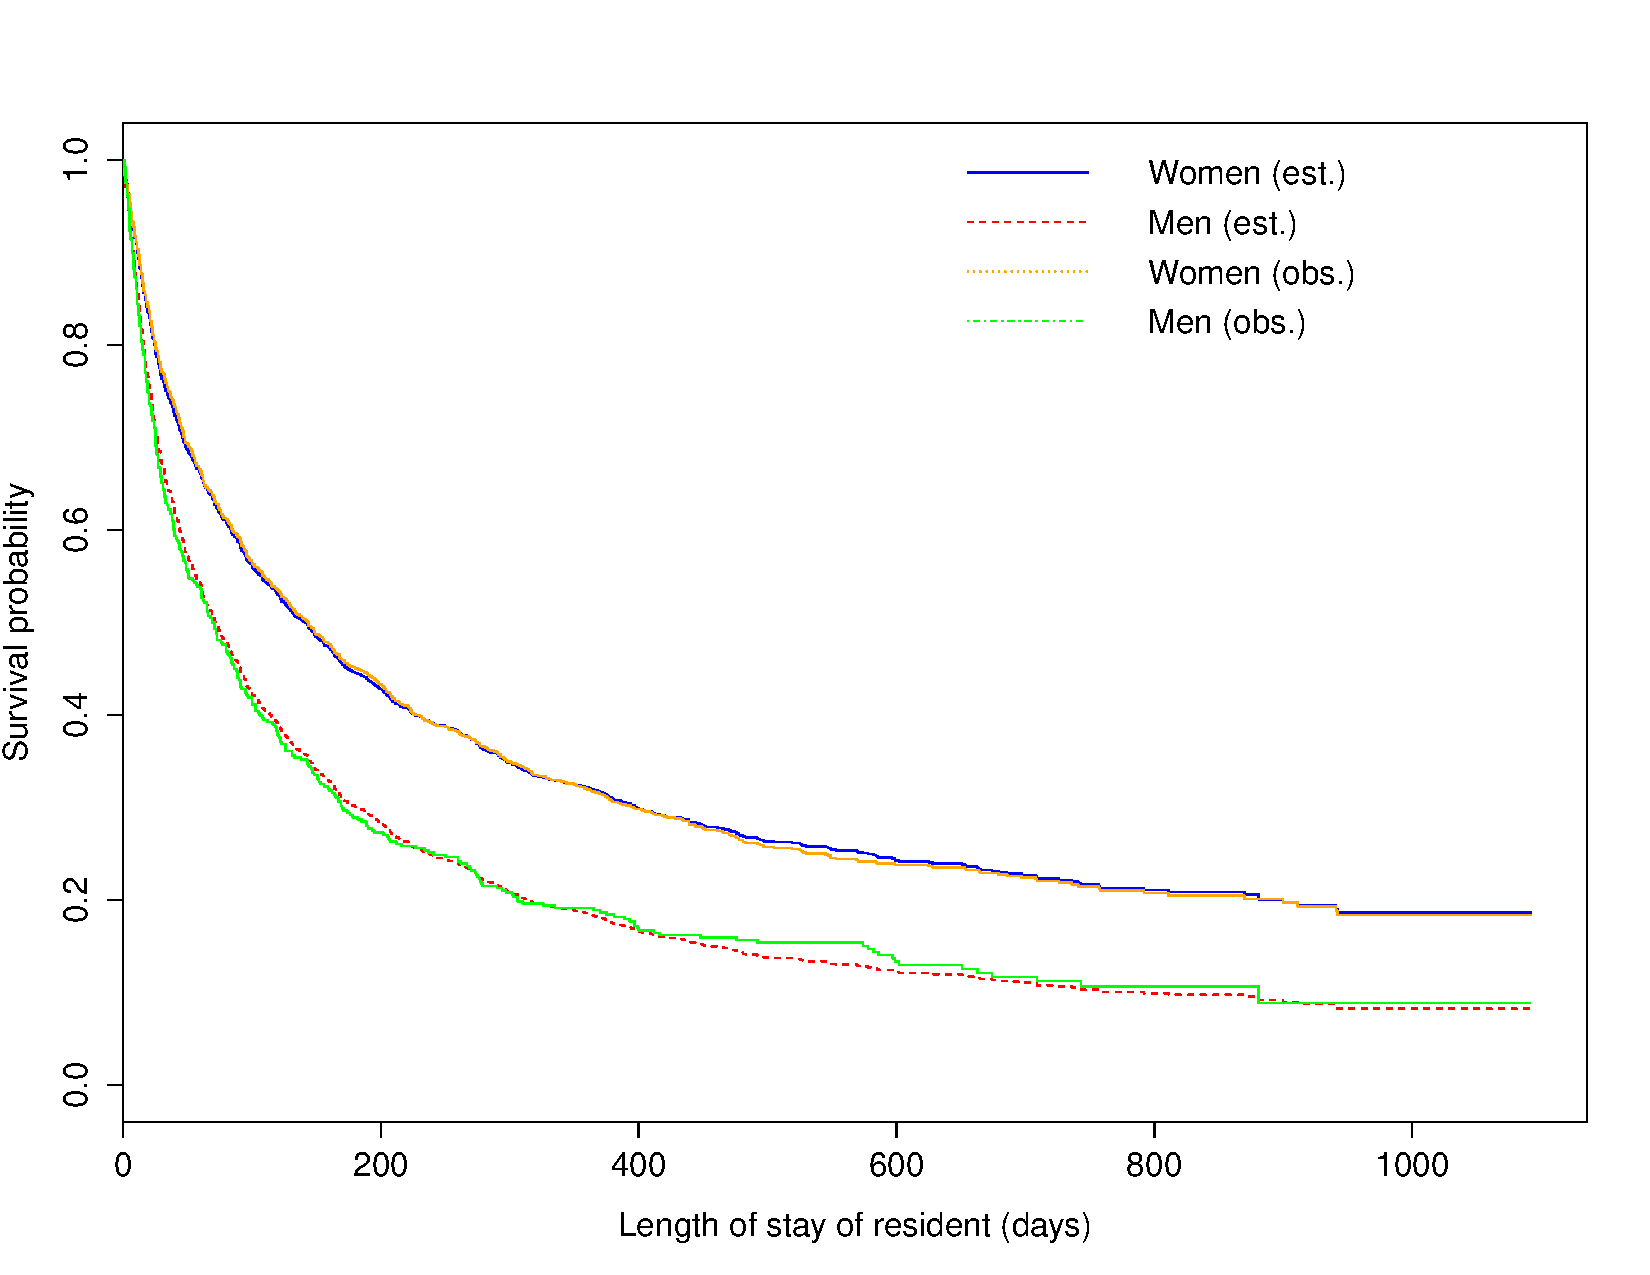
\includegraphics[width=3in]{ch12kmph_sex.pdf}}
\end{frame}
\begin{frame}[fragile]{Assessment of the PH assumption for the combined health/sex effect}
\normalsize
... or for a newly generated covariate (like {\tt hlthsex}) which represents combined
levels of more than one covariate.

\scriptsize
\begin{verbatim}
# Men
# Fit KM curves for males and females
fitKMgr.males = survfit( Surv(los,fail) ~ hlthsex,data = subset(nurshome2, gender==1))

# Compare fitted with observed survival curves for gender
fitCoxgen.males = survfit( coxph( Surv(los,fail) ~ hlthsex, data = nurshome2),
                      newdata = data.frame(hlthsex = as.factor(c("Healthier Men","Sicker Men"))))

plot(fitKMgr.males, mark.time = F,
     xlab = "Length of Stay (days)",ylab = "Survival probability",
     lty = 1:2,col = c("blue","red"))
# Add the raw curves
lines(fitCoxgen.males, lty = 1:2,col = c("green","orange"),mark.time = F)
legend("topright",bty = "n",lty = 1:4,col = c("blue","red","green","orange"),
       legend = c("Predicted: Healthier Men","Sicker Men"),ncol = 1,cex = 0.9)
\end{verbatim}
\end{frame}

\begin{frame}{Health and marital status}

The results are as follows:
\begin{center}
\begin{tabular}{cc}
{\bf Men} & {\bf Women}\\
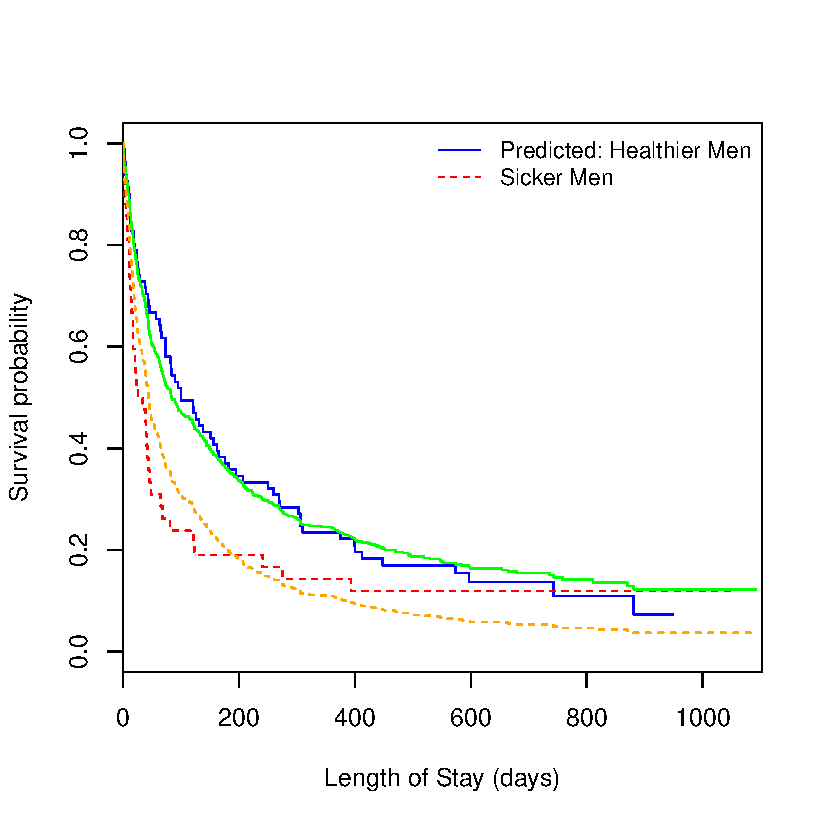
\includegraphics[width=2in]{ch12kmph_males.pdf} &
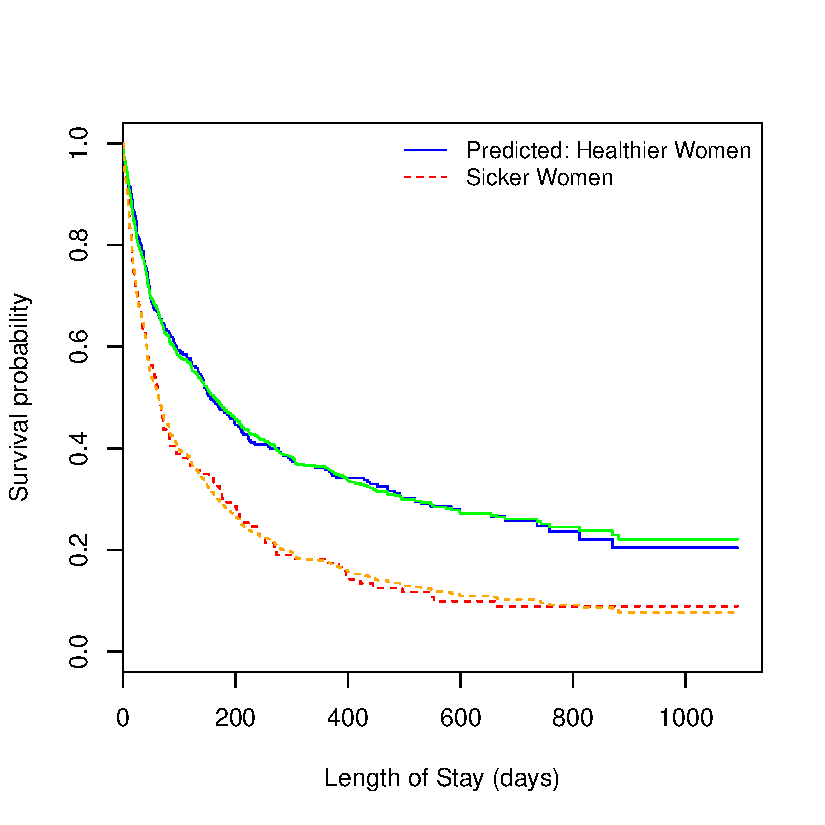
\includegraphics[width=2in]{ch12kmph_females.pdf}
\end{tabular}
\end{center}
The comparison appears to be much better among women than among men.
\end{frame}
\end{document}